\section{Entwicklung eines Taschenrechners}
\label{sec:Taschenrechner}
In dieser Aufgabe soll ein Taschenrechner basierend auf den Grundlagen und Modulen aus den vorangegangen Kapiteln (insbesondere \emph{Adder} und \emph{Multiplier}) durch Hardwarebeschreibung und Implementierung auf dem Basys2 Board realisiert werden. Es handelt sich hierbei um eine \emph{optionale} Aufgabe und hat keinen Einfluss auf die Benotung des Praktikums.
\stoptocwriting
\subsection{\textsc{Versuchsbeschreibung}}

\subsubsection*{Ablaufdiagramm und Spezifikation des Taschenrechners}
In Abbildung \ref{fig:ablauftaschenrechner} ist das Ablaufdiagramm für den zu entwickelnden Taschenrechner gegeben. Das Diagramm kann als Spezifikation der zu realisierenden Hardware verstanden werden, da es das erwartete Verhalten beschreibt. Einen \texttt{Divider} finden Sie unter:\\
\texttt{\centerline {\netzwerkpfadSource/modules}}
\begin{figure}[h!]
\centering
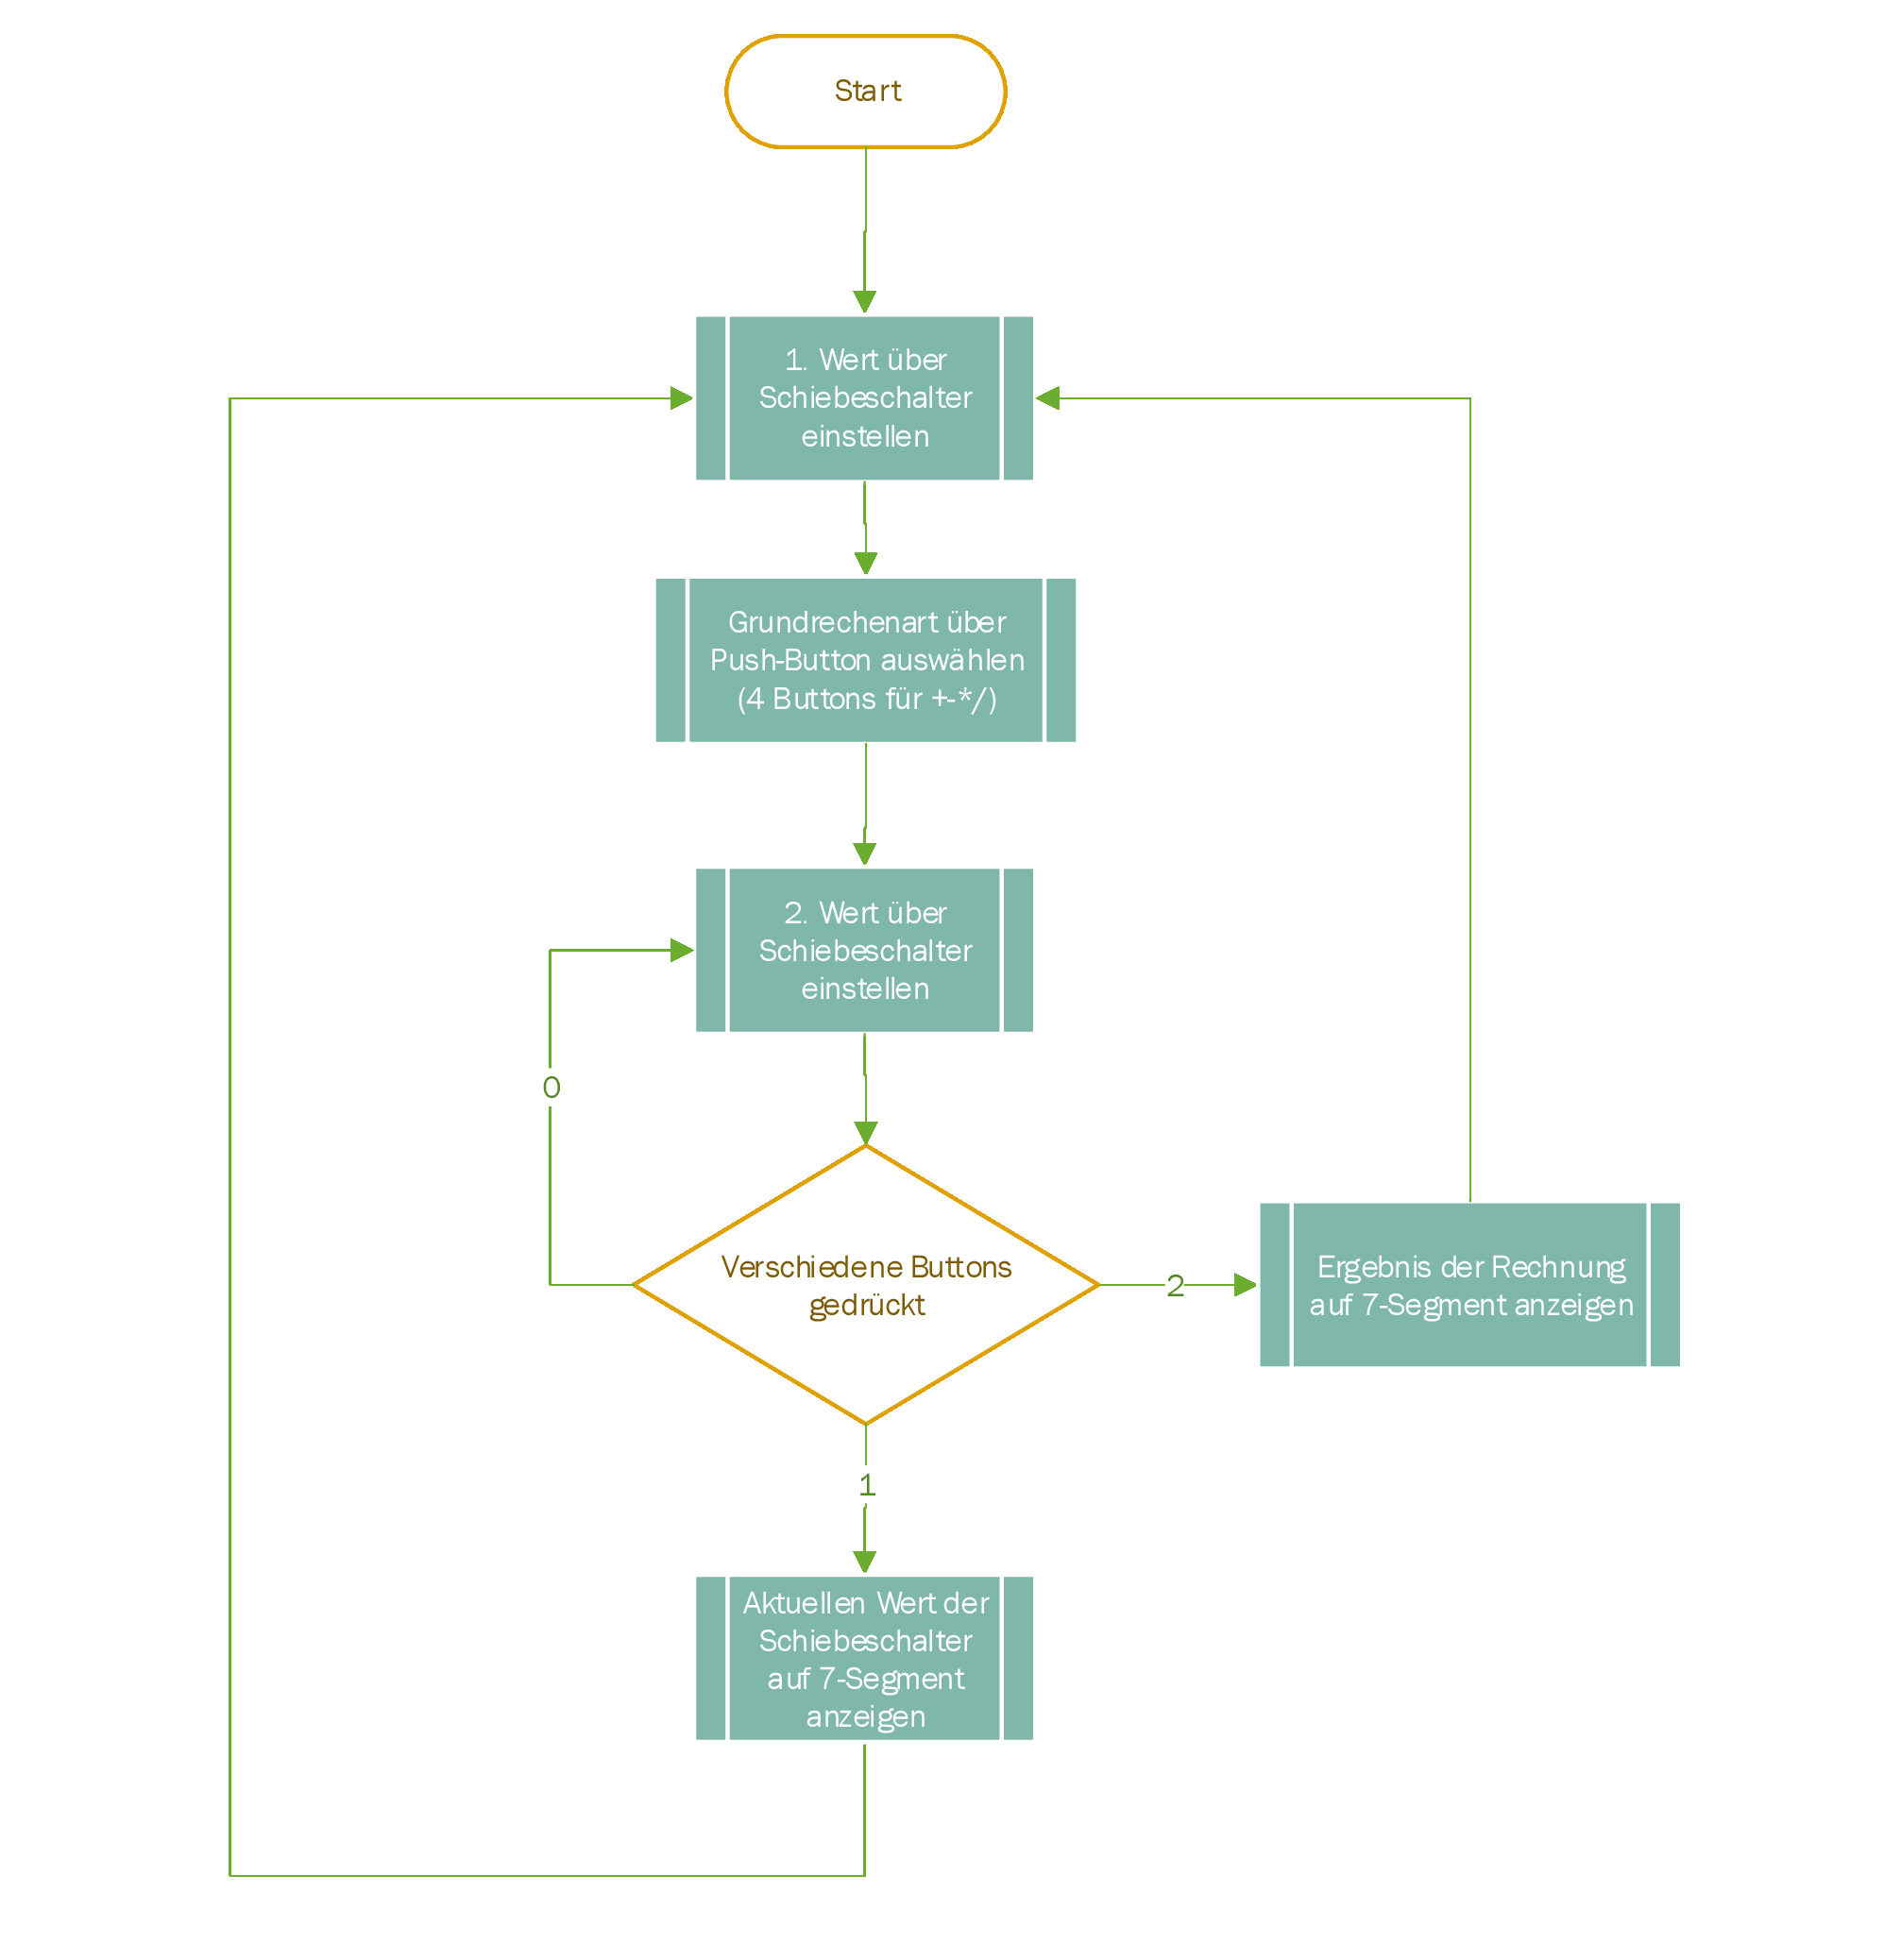
\includegraphics[max height=130mm]{img/Taschenrechner/Ablauf_Taschenrechner}
\caption{Ablaufdiagramm des Taschenrechners}
\label{fig:ablauftaschenrechner}
\end{figure}
\subsection{\textsc{Aufgaben}}
\subsubsection{Grundlegende Überlegungen}
\begin{enumerate}
\item Überlegen Sie sich, inwieweit die Funktion des Taschenrechners beschrieben ist und finden Sie nicht abgedeckte Abläufe!
\item Welche Freiheitsgrade ergeben sich für Sie als Entwickler? Was muss beachtet werden?
\end{enumerate}
\subsubsection{Zustandsautomat des Taschenrechners}
Im nächsten Schritt soll ein endlicher Zustandsautomat anhand der Spezifizierung entwickelt werden, welcher später für die Steuerung des Taschenrechners in Verilog implementiert werden soll.
Die Grundlagen dieser Automaten sind u.a. aus der Vorlesung Mikroelektronik 1 und 2 bekannt. 
\begin{enumerate}
\item Wie viele Zustände besitzt Ihr endlicher Automat (Moore oder Mealy)?
\item Zeichnen Sie den Ihren Entwurf!
\item Für die weiteren Schritte ist ein \texttt{Counter} notwendig. Erläutern Sie warum!
\end{enumerate}
\subsubsection{Blockschaltbild}
Nachdem der Zustandsautomat und somit die Steuerung des Taschenrechners entwickelt wurde, soll ein Blockschaltbild entworfen werden. Das Schaltbild muss ebenfalls die Top-Level Pins (Portliste) enthalten, wobei das Design modular aufgebaut werden soll.\\
Entwerfen Sie ein Blockdiagramm unter Beachtung folgender Punkte:
\begin{itemize}
\item Überdenken Sie Ihren Zustandsautomaten und passen Sie ihn gegebenenfalls an.
\item Verwenden Sie Ihre Module aus den vorangegangenen Kapiteln. Parametrisieren Sie auch die Bitbreiten der einzelnen Ports 
\end{itemize}
\subsubsection{Implementierung und Simulation}
\begin{enumerate}
\item Legen Sie ein neues Projekt in \emph{ISE} an und Implementieren Sie den Taschenrechner. 
\item Testen Sie Ihr (Teil-) Design ausgiebig in einer Simulation. Welche Tests sind sinnvoll? Wie kann solch ein Test automatisiert werden?
\item Validieren Sie Ihr Design auf dem Basys2 Board!
\end{enumerate}
%\subsubsection{\textit{Optional:} Überlauferkennung, soll noch entschieden werden, zeitabhängig...}
\resumetocwriting